% !TEX TS-program = pdflatexmk

\documentclass[a4paper, twoside]{article}

\usepackage{color}
\usepackage{graphicx}
\usepackage[colorlinks]{hyperref}

\begin{document}

\title{Burden of Proof demo1b \\ Game Design Document}

\maketitle

\tableofcontents

\newpage

\section{Game}

\subsection{Overview}

\begin{itemize}
	\item{} genre : crime investigation video game ;
	\item{} demographics : 16+ ;
	\item{} TODO.
\end{itemize}

\newpage

\subsection{Gameplay}

TODO

\newpage

\subsection{City design}

City built from blueprint using parts specified in figure~\ref{fig:cityparts}.

\begin{figure}[h!tbp]
	\centering
	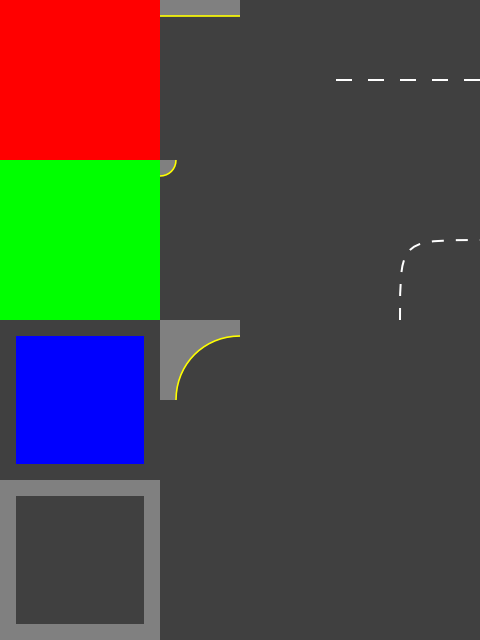
\includegraphics[width=0.8\textwidth]{images/cityparts.png}\ 
	\caption{City parts
		- First column : road block, ground block, building block, building pad
		- Second column : half sidewalk, interior sidewalk, exterior sidewalk
		- Third column : sraight markings, curved markings
		- Sidewalks have a roadside curb (yellow)}
	\label{fig:cityparts}
\end{figure}

\newpage

\section{Implementation}

\subsection{Code design}

\begin{figure}[h!tbp]
	\centering
	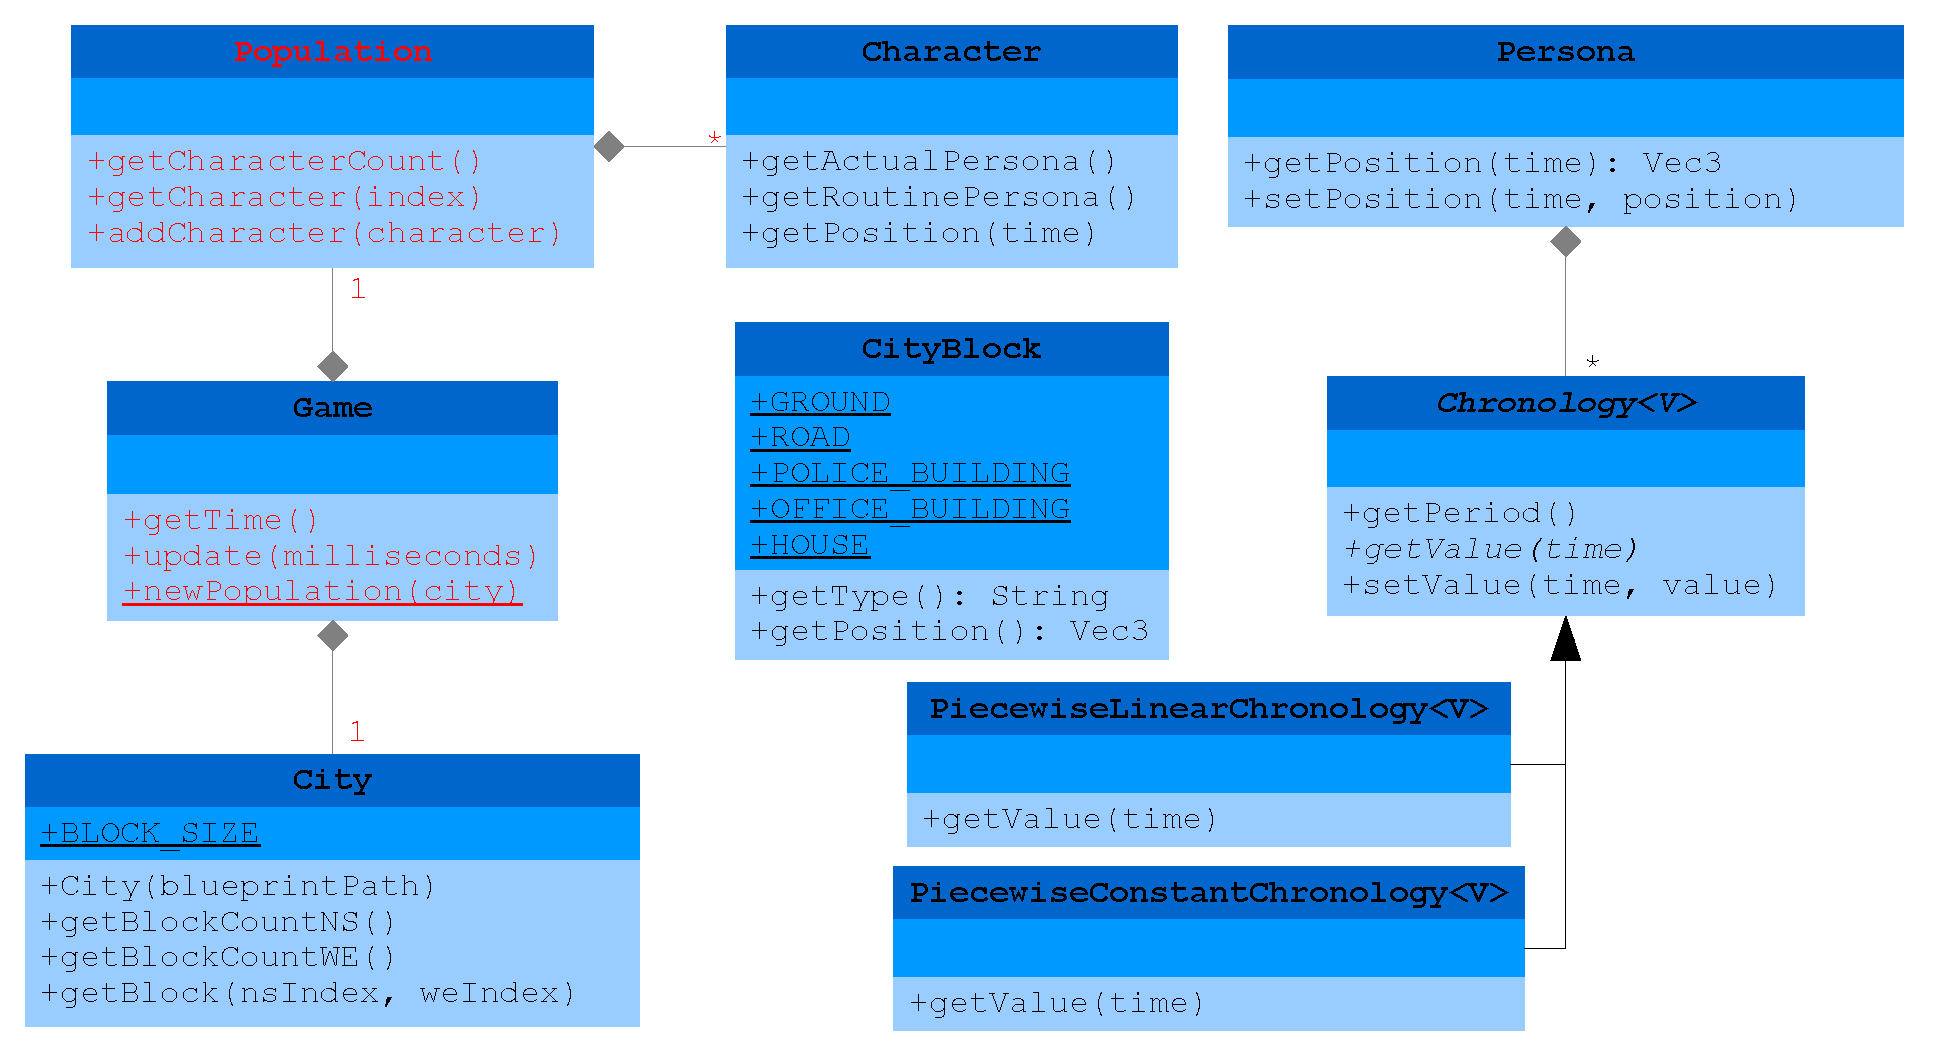
\includegraphics[width=1.0\textwidth]{images/classes.pdf}\ 
	\caption{Classes}
	\label{fig:classes}
\end{figure}

TODO: more UML diagrams

\newpage

\subsection{Coding conventions}

\begin{itemize}
	\item{} C++: cpplint
	\item{} Python: pep8
\end{itemize}

\newpage

\subsection{Planning}

\begin{enumerate}
	\item{} \textcolor{black}{Application} \begin{enumerate}
		\item{} \textcolor{black}{(DONE) Setup project files}
		\item{} \textcolor{black}{(DONE) Add basic application code from demo1}
	\end{enumerate}
	\item{} \textcolor{black}{Model - Essential classes} \begin{enumerate}
		\item{} \textcolor{black}{(DONE) Design (figure~\ref{fig:classes})}
		\item{} \textcolor{black}{(DONE) Test and implement}
		\item{} \textcolor{black}{(DONE) Integrate with application}
	\end{enumerate}
	\item{} \textcolor{red}{Model - Crime generation} \begin{enumerate}
		\item{} \textcolor{red}{(TODO) Generate more detailed routine motion paths}
		\item{} \textcolor{red}{(TODO) Add method Game.generateCrime() with Persona attribute murderousIntent}
	\end{enumerate}
	\item{} \textcolor{red}{Graphics - City} \begin{enumerate}
		\item{} \textcolor{black}{(DONE) Integrate city parts generation from demo1}
		\item{} \textcolor{black}{(DONE) Integrate city generation from demo1}
		\item{} \textcolor{blue}{(codistmonk) Integrate city visualization from demo1}
		\item{} \textcolor{red}{(TODO) Add skybox (blue sky + sun)}
		\item{} \textcolor{red}{(TODO) Add trees}
		\item{} \textcolor{red}{(TODO) Add streetlights}
		\item{} \textcolor{red}{(TODO) Add buildings}
	\end{enumerate}
	\item{} \textcolor{red}{Graphics - Characters} \begin{enumerate}
		\item{} \textcolor{red}{(TODO) Update orientation during motion}
		\item{} \textcolor{red}{(TODO) Integrate character generation from generatehuman}
		\item{} \textcolor{red}{(TODO) Add neutral character visualization}
		\item{} \textcolor{red}{(TODO) Add walking animation}
		\item{} \textcolor{red}{(TODO) Add levels of detail}
		\item{} \textcolor{red}{(TODO) Add clothes}
		\item{} \textcolor{red}{(TODO) Add hair}
		\item{} \textcolor{red}{(TODO) Add gender visualization}
		\item{} \textcolor{red}{(TODO) Add age visualization}
		\item{} \textcolor{red}{(TODO) Add ethnicity visualization}
	\end{enumerate}
	\item{} \textcolor{red}{Graphics - Phone} \begin{enumerate}
		\item{} \textcolor{red}{(TODO) Add phone visualization and control from demo1}
		\item{} \textcolor{red}{(TODO) Add time display to phone}
	\end{enumerate}
	\item{} \textcolor{red}{Investigation} \begin{enumerate}
		\item{} \textcolor{red}{(TODO) Design and planning}
	\end{enumerate}
\end{enumerate}

\end{document}
